\documentclass[]{article}

\usepackage[utf8]{inputenc}
\usepackage[T1]{fontenc}
\usepackage{graphicx}
\usepackage{geometry}
\usepackage{svg}
\setsvg{inkscapeversion=1.4}

\geometry{headheight=0cm, top=2.5cm, bottom=3cm}

\begin{document}

\title{\textbf{ Werkzeuge für das wissenschaftliche Arbeiten}\\
 \normalsize Python for Machine Learning and Data Science}
\date{Abgabe: 15.12.2023}
\maketitle

\renewcommand{\contentsname}{Inhaltsverzeichnis} 
\tableofcontents 

\vspace{1em}

\setcounter{secnumdepth}{0} 
\section{1. Projektaufgabe}
In dieser Aufgabe beschäftigen wir uns mit Objektorientierung in Python. Der Fokus liegt auf der Implementierung einer Klasse, wobei wir insbesondere auch Magic Methods nutzen.\\

\renewcommand{\figurename}{Abbildung}
\begin{figure}[htbp]
  \centering
  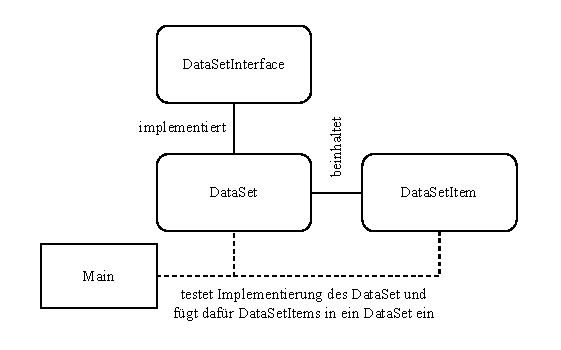
\includegraphics[width=\textwidth]{../diagram/classes_files.pdf}
  \caption{Darstellung der Klassenbeziehungen.\normalsize}
\end{figure}

\subsection{1.1 Einleitung}
Ein Datensatz besteht aus mehreren Daten, ein einzelnes Datum wird durch ein Objekt der Klasse "DataSetItem" repräsentiert. Jedes Datum hat einen Namen (Zeichenkette), eine ID (Zahl) und bel. Inhalt. \\
Nun sollen mehrere Daten, Objekte vom Typ "DataSetItem", in einem Datensatz zusammengefasst werden. Sie haben sich schon auf eine Schnittstelle und die benötigten Operationen, die ein Datensatz unterstützen muss, geeinigt. Es gibt eine Klasse "DataSetInterface", die die Schnittstelle definiert und Operationen jedes Datensatzes angibt. Bisher fehlt aber noch die Implementierung eines Datensatzes mit allen Operationen. 
\\
Implementieren Sie eine Klasse "DataSet" als eine Unterklasse von "DataSet- Interface".

\subsection{1.2 Aufbau}
Es gibt drei Dateien, \texttt{dataset.py}, \texttt{main.py} und \texttt{implementation.py}$^{*}$. In der \texttt{dataset.py} befinden sich die Klassen \texttt{DataSetInterface} und \texttt{DataSetItem}, in der Datei \texttt{implementation.py} muss die Klasse \texttt{DataSet} implementiert werden. Die Datei \texttt{main.py} nutzt die Klassen \texttt{DataSet} und \texttt{DataSetItem} aus den jeweiligen Dateien und testet die Schnittstelle und Operationen von \texttt{DataSetInterface}.\\

\subsection{1.3 Methoden}
Bei der Klasse \texttt{DataSet} sind insbesondere folgende Methoden zu implementieren, die genaue Spezifikation finden Sie in der \texttt{dataset.py}:
\begin{itemize}
    \item \texttt{\_\_setitem\_\_(self, name, id\_content)}: Hinzufügen eines Datums mit Name, ID und Inhalt
    \item \texttt{\_\_iadd\_\_(self, item)}: Hinzufügen eines \texttt{DataSetItem}
    \item \texttt{\_\_delitem\_\_(self, name)}: Löschen eines Datums basierend auf dem Namen
    \item \texttt{\_\_contains\_\_(self, name)}: Prüfen, ob ein Datum mit diesem Namen im Datensatz vorhanden ist
    \item \texttt{\_\_getitem\_\_(self, name)}: Abrufen des Datums über seinen Namen
    \item \texttt{\_\_and\_\_(self, dataset)}: Schnittmenge zweier Datensätze bestimmen und als einen neuen Datensatz zurückgeben
    \item \texttt{\_\_or\_\_(self, dataset)}: Vereinigung zweier Datensätze bestimmen und als einen neuen Datensatz zurückgeben
    \item \texttt{\_\_iter\_\_(self)}: Iteration über alle Daten des Datensatzes (mit optionaler Sortierung)
    \item \texttt{filtered\_iterate(self, filter)}: Gefilterte Iteration über einen Datensatz, wobei eine Lambda-Funktion mit den Parametern Name und ID für jedes Datum als Filter dient
    \item \texttt{\_\_len\_\_(self)}: Anzahl der Daten in einem Datensatz abrufen
\end{itemize}

\section{2. Abgabe}
Programmieren Sie die Klasse \texttt{DataSet} in der Datei \texttt{implementation.py} zur Lösung der oben beschriebenen Aufgabe im VPL. Die benötigten Dateien können auch direkt auf Ihrem Computer heruntergeladen werden. Das VPL nutzt denselben Code, wobei die \texttt{main.py} um weitere Testfälle und Überprüfungen erweitert wurde. Diese Überprüfungen dienen dazu sicherzustellen, dass Sie die richtigen Klassen nutzen. 
\footnote{$^{*}$ Die Dateien befinden sich im Ordner "/code/" dieses Git-Repositories.}

\end{document}
